\documentclass[a4paper,12pt]{article}
\usepackage[left=2.5cm,right=2.5cm,top=2.5cm,bottom=2.5cm]{geometry} % Adjust page margins
\usepackage{xcolor,graphicx,framed}
\usepackage[normalem]{ulem}
\usepackage{amsmath}
\usepackage{gensymb}
\usepackage{chemmacros}
%\usepackage{lastpage} % Required to print the total number of pages

\begin{document}

\newcommand{\HRule}{\rule{\linewidth}{0.4mm}} % Defines a new command for the horizontal lines, change thickness here

%----------------------------------------------------------------------------------------
%	HEADING SECTIONS
%----------------------------------------------------------------------------------------

\begin{minipage}{0.7\textwidth}
\begin{flushleft} 
\textsc{Universidad del Valle de Guatemala \\
Campus Central \\
Facultad de Ciencias y Humanidades \\
Departamento de Qu\'imica \\
Segundo ciclo, 2014 \\
Fisicoqu\'imica 1 \\
Secci\'on 20
}
\end{flushleft}
\end{minipage}
~
\begin{minipage}{0.2\textwidth}
\begin{flushright}

\includegraphics[scale=0.3]{Logo_UVG} % Include a department/university logo
\end{flushright}
\end{minipage}\\

%----------------------------------------------------------------------------------------
%	TITLE SECTION
%----------------------------------------------------------------------------------------

\begin{center}
\HRule \\[0.4cm]
{ \bfseries Evaluaci\'on 3}\\ % Title of your document
\HRule \\[0.4cm]
\end{center}

%----------------------------------------------------------------------------------------

\section*{Instrucciones}

Responder y resolver los siguientes problemas en las hojas adicionales haciendo uso de calculadora cient\'ifica, una tabla peri\'odica y el libro de texto que hayan tra\'ido. Cualquier actitud deshonesta ser\'a sancionada seg\'un el C\'odigo de comportamiento de los estudiantes de la Universidad.

\section*{Problemas}

\begin{enumerate}

 \item (10 pts) La siguiente figura muestra el comportamiento de la presi\'on de vapor de tres soluciones, en el rango de distintas composiciones. Indicar cu\'al es la que se comporta como una soluci\'on ideal e indicar c\'omo entender las desviaciones de las otras dos, utilizando la idea de fuerzas intermoleculares.

\begin{center}
 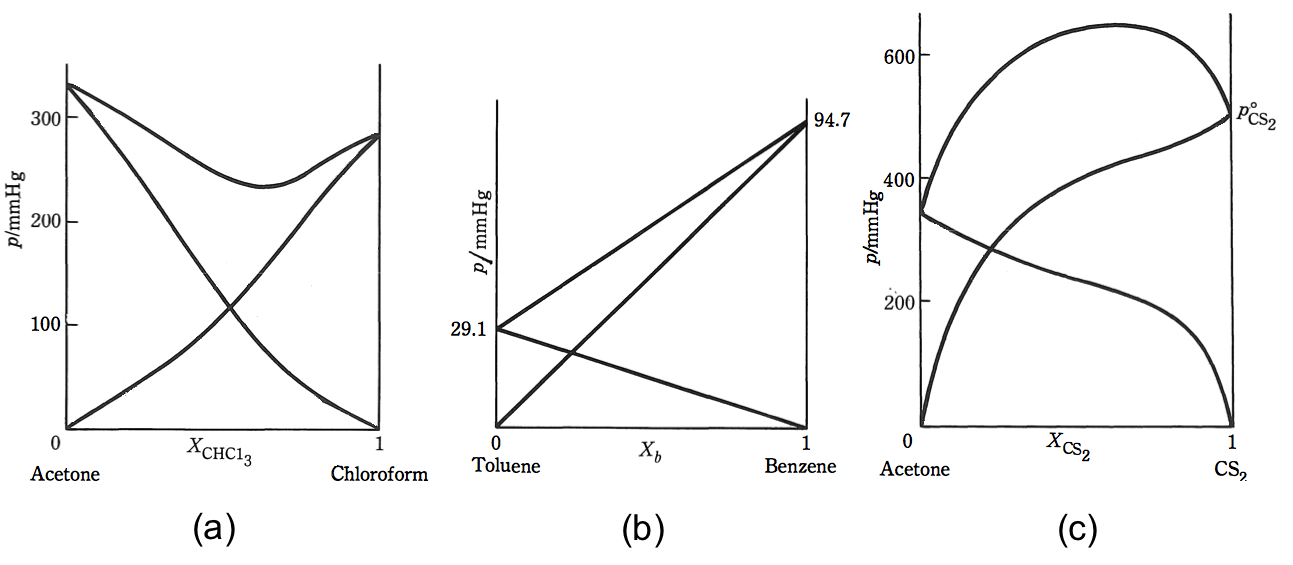
\includegraphics[scale=0.3]{figure1}
\end{center} % Problema de ley de Raoult

 \item (30 pts) Construir el diagrama de fase para el benceno cercano al punto triple ($5.50\,\celsius$ y $36\;\mbox{torr}$) usando la siguiente informaci\'on: $\Delta_{fus}H=10.6\;\mbox{kJ}\cdot\mbox{mol}^{-1}$, $\Delta_{vap}H=30.8\;\mbox{kJ}\cdot\mbox{mol}^{-1}$, $\rho(s)=0.891\;\mbox{g}\cdot\mbox{cm}^{-3}$, $\rho(l)=0.897\;\mbox{g}\cdot\mbox{cm}^{-3}$. % Problema 4.10 de Atkins

 \item (20 pts) La presi\'on de vapor de un l\'iquido entre $15\,\celsius$ y $35\,\celsius$ se comporta seg\'un la ecuaci\'on $\log(P/\mbox{torr})=8.750-1625/(T/\mbox{K})$. Calcular la entalp\'ia de vaporizaci\'on y el punto de ebullici\'on normal del l\'iquido. % Problema 4.11(b) de Atkins

 \item (20 pts) Considere la s\'intesis del diamante a partir de grafito:
$$\mbox{C(grafito)}\;\rightarrow\;\mbox{C(diamante)}$$
 \begin{enumerate}
  \item Calcular los valores de $\Delta_r\bar{H}^\standardstate$ y $\Delta_r\bar{S}^\standardstate$.
  \item Determinar si la reacci\'on ocurre espont\'aneamente a $25\,\celsius$. Si no, ?`hay alguna temperatura en la cual sea espont\'anea?
  \item Con base en las mediciones de densidad, se ha encontrado que el volumen molar del grafito es $2.1\;\mbox{cm}^3$ mayor que el del diamante. ?`Se puede efectuar la conversi\'on de grafito a diamante aproximadamente a $25\,\celsius$ aplicando presi\'on sobre \'el? De ser as\'i, determinar la presi\'on a la cual el proceso se hace espont\'aneo.
 \end{enumerate} % Problema 6.8 de Chang 

 \item (20 pts) Los vol\'umenes molares parciales de dos l\'iquidos $A$ y $B$, en una mezcla para la cual la fracci\'on molar de $A$ es $0.3713$, son $188.2\;\mbox{cm}^3\cdot\mbox{mol}^{-1}$ y $176.14\;\mbox{cm}^3\cdot\mbox{mol}^{-1}$, respectivamente. Las masas molares de $A$ y $B$ son $241.1\;\mbox{g}\cdot\mbox{mol}^{-1}$ y $198.2\;\mbox{g}\cdot\mbox{mol}^{-1}$. ?`Cu\'al es el volumen de una soluci\'on de $1.000\;\mbox{kg}$ de masa total? % Problema 5.2(b) de Atkins

\end{enumerate}

\end{document}
